\documentclass[12pt]{article}
\usepackage{amsmath}
\usepackage{amssymb}
\usepackage{amsthm}
\usepackage{amsfonts}
\usepackage{graphicx}
\usepackage{textcomp}
\usepackage{hyperref}
\usepackage{tikz}
\usepackage{enumitem}
\usepackage{mathtools}
\usepackage{float}

\begin{document}

\title{Discrete Mathematics 1 - Logical Equivalences}
\author{Alexander Ng}
\date{September 13, 2024}

\maketitle

\begin{figure}[H]
    \centering
    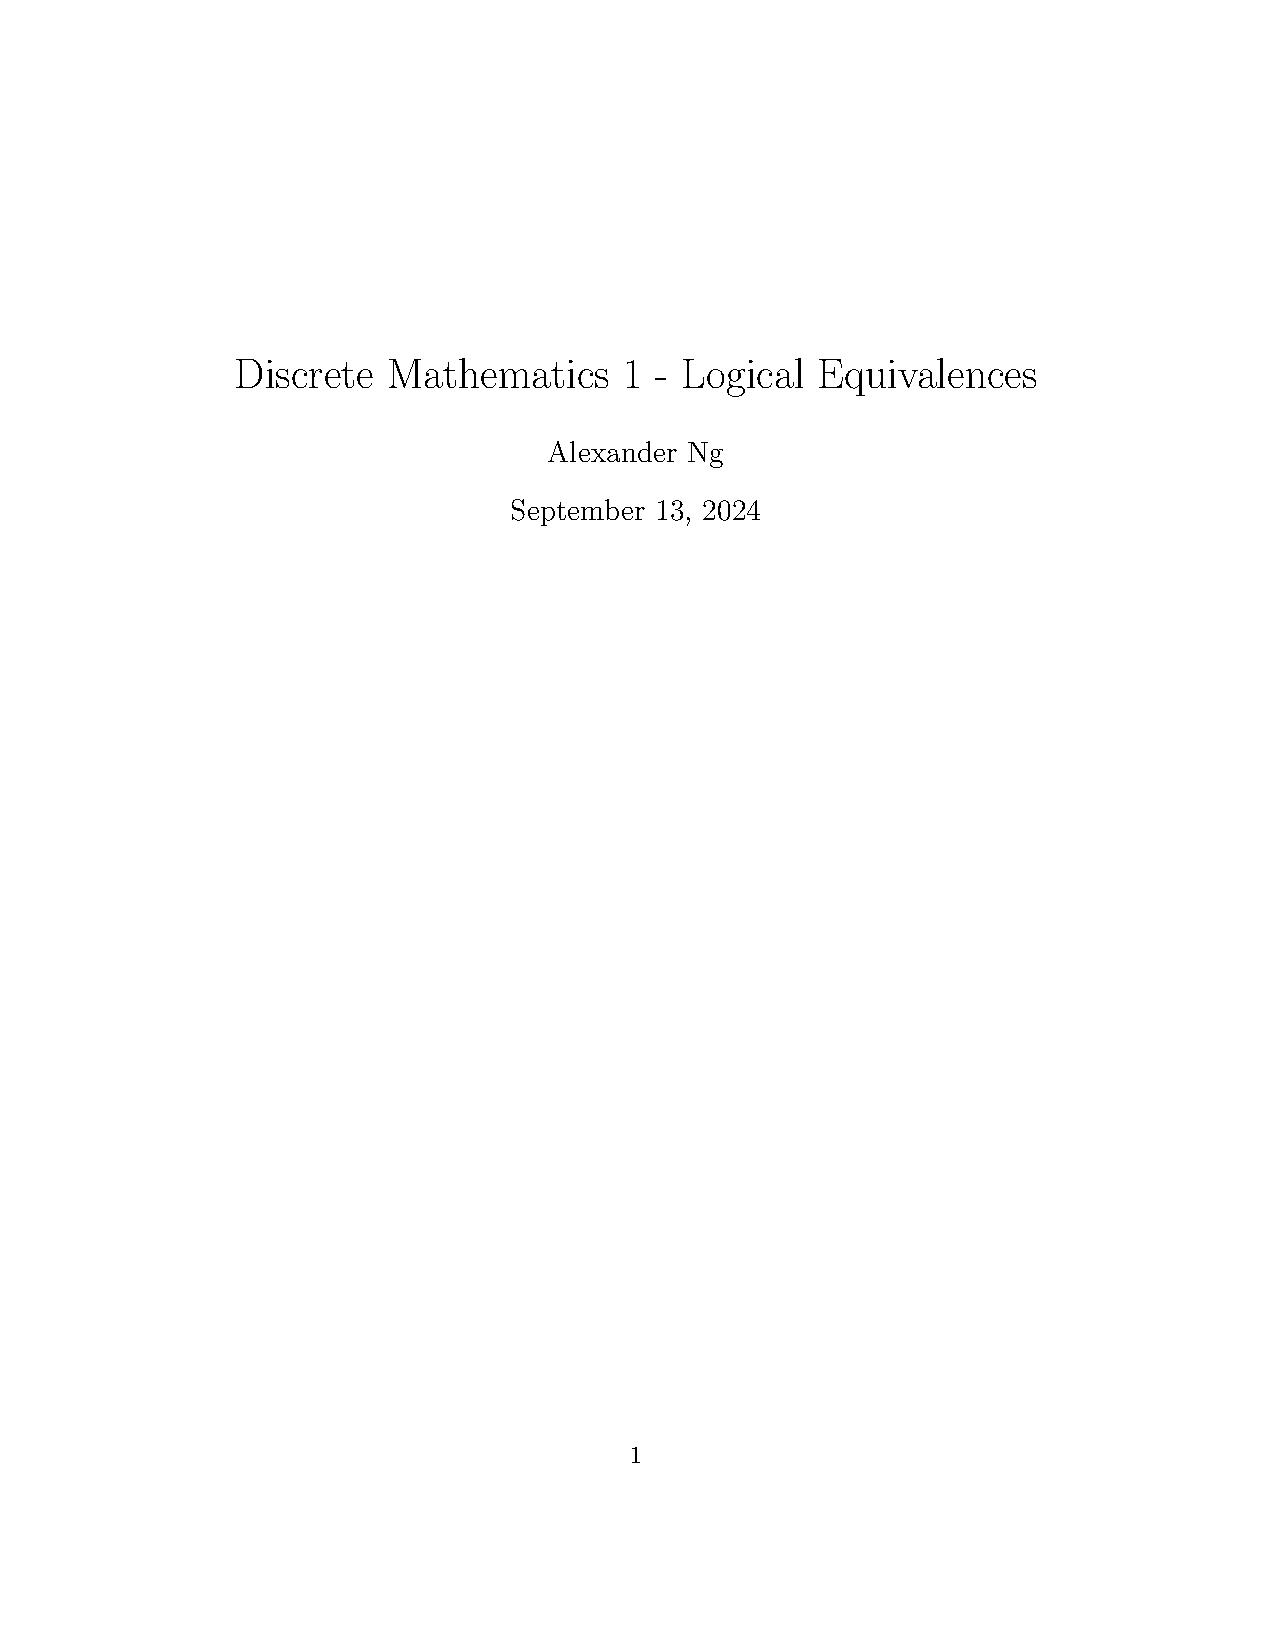
\includegraphics[width=0.8\textwidth]{"./Logical Equivalences.jpg"}
    \caption{Logical Equivalences}
\end{figure}

\begin{figure}[H]
    \centering
    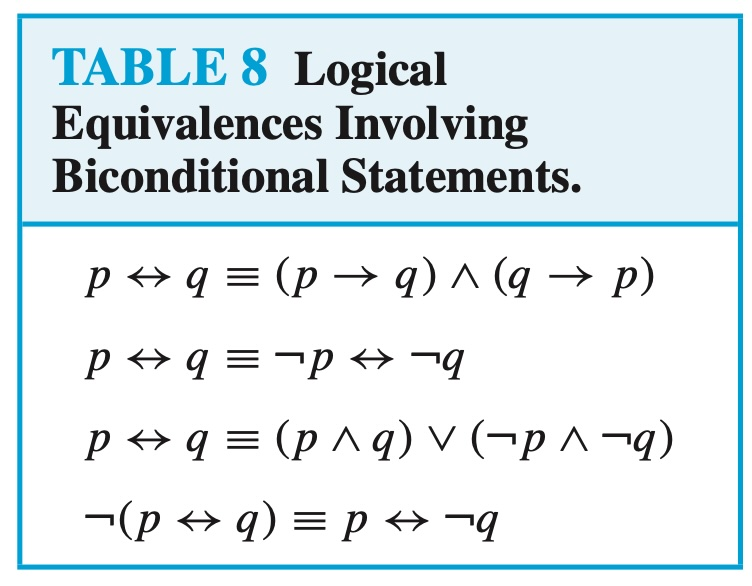
\includegraphics[width=0.4\textwidth]{"./Logical Equivalences Involving Biconditional Statements.jpg"}
    \caption{Logical Equivalences Involving Biconditional Statements}
\end{figure}

\begin{figure}[H]
    \centering
    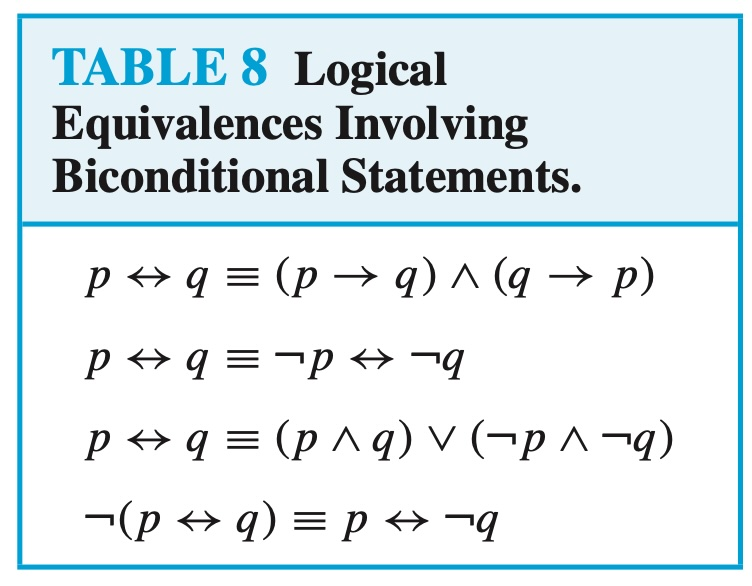
\includegraphics[width=0.4\textwidth]{"./Logical Equivalences Involving Biconditional Statements.jpg"}
    \caption{Logical Equivalences Involving Conditional Statements}
\end{figure}


\end{document}
